%&program=xelatex
%&encoding=UTF-8 Unicode
% SVN keywords
% $Author$
% $Date$
% $Revision$
% $URL$
\documentclass[a4paper,twoside,12pt]{article}      % Comments after  % are ignored
%\usepackage{hyperref}                 % For creating hyperlinks in cross references
%\documentclass[a4paper,12pt]{article} 
%
%\usepackage{yhmath}
%\pdfmapfile{yhmath.map} %without this pk-fonts are used


\usepackage{ifxetex}% for XELATEX, or PDFlatex
\usepackage{ifplatform} 
%
\ifxetex
\usepackage{polyglossia} \setmainlanguage{portuges}
\usepackage{fontspec}
\ifwindows
\setmainfont{Garamond}
\setsansfont{Gill Sans MT}
\setmonofont[Scale=MatchLowercase]{Courier}
\fi
\iflinux
\setmainfont[Ligatures=TeX]{Linux Libertine O}
\setsansfont[Ligatures=TeX,Scale=MatchLowercase]{Linux Biolinum}
\setmonofont[Scale=MatchLowercase]{Courier}
\fi
\ifmacosx
% add settings
\fi
%
\usepackage{xcolor,graphicx} 
\else
%PdfLaTEX
\usepackage[portuguese]{babel}
\usepackage[utf8]{inputenc}
\usepackage[T1]{fontenc}
\usepackage{graphics}                 % Packages to allow inclusion of graphics
\usepackage{color}                    % For creating coloured text and background
\fi

\usepackage{amsmath,amssymb,amsfonts} % Typical maths resource packages

\oddsidemargin 0cm
\evensidemargin 0cm

\pagestyle{myheadings}         % Option to put page headers
                               % Needed \documentclass[a4paper,twoside]{article}
\markboth{{\small\it MEFT - 2013/2014}}
{{\small\it Laboratório de Física Experimental Básica}}

\textwidth 15.5cm
\topmargin -1cm
\parindent 0cm
\textheight 24cm
\parskip 1mm


%\setmainfont[Ligatures=TeX]{Hoefler Text} 
%\setmainfont[Ligatures=TeX]{Times}
%\setsansfont[Ligatures=TeX,Scale=MatchLowercase]{Gill Sans} \setmonofont[Scale=MatchLowercase]{Courier}
%\setromanfont[Numbers=Uppercase]{Hoefler Text}
%\usepackage{xcolor,graphicx} 

%[pdftex]
%\usepackage{amsmath,amssymb} 
%\usepackage{amsmath} 
%\usepackage{textcomp}

% Math macros
\newcommand{\ud}{\,\mathrm{d}} 
\newcommand{\HRule}{\rule{\linewidth}{0.5mm}}

%\title{ e Difracção de Ondas Electromagnéticas num meio dieléctrico, homogéneo e isotrópico } 
%\subtitle{ aplicação à luz visível} 

\author{Prof. Bernardo B. Carvalho} 

%, Bernardo Brotas Carvalho\\bernardo@ipfn.ist.utl.pt} 
\date{ Setembro 2012} 

\begin{document} 

%	\begin{center}
%	\textsc{\large Laboratório de Física Experimental Básica - MEFT - 2012/2013 }\\%[0.5cm]
%	\end{center}

\includegraphics[width=0.2\textwidth]{./logo-ist}%\\[1cm]  %%  Logo_IST_color
	
	\HRule \\[0.5cm]
	{ \huge   \bfseries \textsc{ Pendulo Gravítico } }\\[0.4cm]
	{ \large \bfseries Determinação do período do pêndulo simples e aferição com o valor da Aceleração da Gravidade local $g$  }\\
%	{ \large \begin{flushleft}
%	 $\bullet$ Deflexão magnética \\
%	 $\bullet$ Deflexão magnética em equilíbrio com deflexão eléctrica
%	\end{flushleft} }
	\HRule \\%[0.5cm]
%	\textsc{\Large Laboratório de Física Experimental Básica}\\[0.5cm]
	
%	\input{./title_exa.tex} 

%\maketitle
%\section{\sf  Conceitos necessários:} 
%\begin{enumerate}
%	\item Força eléctrica. Campo eléctrico (Electrostático)
%	\item Potencial eléctrico. Equipotencial. Energia potencial eléctrica 
%	\item Condutores e dieléctricos. Condensador plano
%	\item Efeitos da corrente eléctrica estacionária criada por uma espira 	
%	\item Força de Laplace
%\end{enumerate}

\section{\sf Movimento Harmónico Simples}

O Pêndulo Gravítico é um exemplo simples do modelo "matemático", o ``Oscilador Harmónico'' (OH), de essencial importância e  vastíssima utilização em quase todos o ramos da Física, bem como muitas áreas de Engenharia. Neste modelo, um sistema físico arbitrário encontra-se inicialmente parado na vizinhança de uma posição de equilíbrio (mínimo da sua Energia Potencial - $E_P$ ). Fora deste mínimo surge sempre uma força de índole conservativa, sempre direcionada de forma a repor o equilíbrio. 
Quando as forças exteriores que mantêm a posição inicial deixam de actuar o sistema adquire movimento, 
transferindo-se a $E_P$ para Energia Cinética ($E_C$). 
Ao atingir a posição de equilíbrio e por inércia o movimento prossegue até se alcançar um novo máximo simétrico. Na ausência de forças dissipativas, o sistema regressa  ao ponto de partida e o ciclo repete-se infinitamente, com período $T_0$ constante (``Oscilador Livre''). Na presença de atrito a Energia Total deixa de ser constante e irá dissipar-se, diminuindo a amplitude do movimento, até desaparecer (``Oscilador Amortecido'').
% \begin{figure}
	% [t!bp]  \centering 
	% \includegraphics[width=0.45	\textwidth]{cucu} 
	% \caption{O Pêndulo gravítico foi até meados do sex. XX a forma mais exacta de medir o tempo. \label{fig:1}} 
% \end{figure}

%, no caso de Mecânica uma massa,
\subsection{\sf Sistema Massa-mola}
O exemplo de modelo OH mecânico mais simples  consiste num sistema de uma massa que se move na horizontal e sem atrito,  presa a uma mola  que é fixada na sua outra extremidade (Figura \ref{fig:2}). Caso a massa se deslocar da posição de equilíbrio ($x =0$), a Energia Potencial Elástica aumenta e mola irá exercer uma força de sinal contrário à deslocação $\Delta x = x - x_0 = x$. No modelo ideal da mola \emph{linear}  a força tem  módulo proporcional (com constante $k_{mola}$) ao deslocamento $x$ 

\begin{equation}
F_{mola} = - k_{mola} \, x \qquad (N)
\end{equation}

A partir da famosa equação de Newton $F=m a$ e sabendo que $ a = \ddot{x}= \frac{d^2 x}{dt^2}$ é possível chegar facilmente  à equação de movimento do sistema Massa-Mola (equação diferencial de 2º grau)

\begin{equation}
	\label{eq:1} 
 m a = - k_{mola} x \Leftrightarrow \frac{d^2 x}{dt^2}  + \frac{k_{mola}}{m} x = 0
\end{equation}

%\Rightarrow
Pode-se verificar em poucos passos que a seguinte função temporal periódica é solução da equação (\ref{eq:1} ).

\begin{equation}
	\label{eq:solu_mola}
x(t) = A_0 \sin(w_0 \, t + \phi_0) \text{, com } w_0 = \sqrt{\frac{k_{mola}}{m}}
\end{equation}

Com $ A_0 $ (Amplitude) e $\phi_0$ (fase) constantes, dependentes da condições iniciais. Finalmente $w_0$ é a frequência angular de ressonância que tal como o período dependem apenas da massa e de $k_{mola}$:
%, $\frac{2 \pi}{T}$,

\begin{equation}
	\label{eq:period_mola}
T_0 = \frac{2 \pi}{w_0} = 2\pi\; \sqrt{\frac{m}{k_{mola}}}	
\end{equation}

Assim, a solução para a posição ( e também para a velocidade, desfasada de $\pi/2$), é uma função sinusoidal (harmónica).

\begin{figure}
	[!tbp] \centering 
	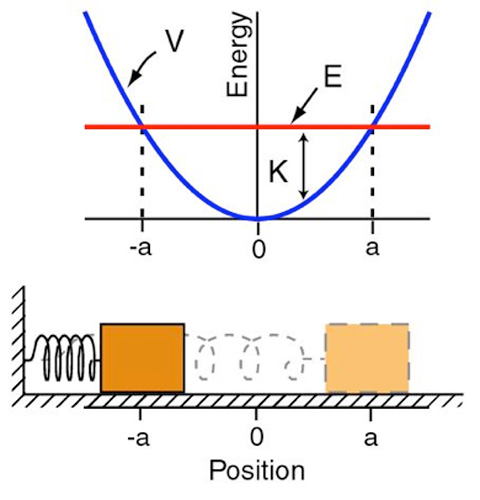
\includegraphics[width=0.5	\textwidth]{simple_harmonic_oscillator} 
	\caption{Oscilador Harmônico Simples \emph{Massa-Mola}.  \label{fig:2}} 
\end{figure}

\subsection{\sf Pêndulo gravítico}
O Pêndulo gravítico é também um sistema que pode ter como modelo o ``Oscilador Harmónico'' e que consiste numa massa pontual suspensa ( do Latim \emph{pendulus}) a partir de um fio, virtualmente sem massa, e comprimento $l$ fixo que pode rodar em torno de um ponto (o ``pivôt"). Quando a massa se desvia da posição central, a força gravítica aplicada em $m$ (o peso $F_g = m \, g $) adquire uma componente na direcção de movimento (tangente à trajectória circular) e que tende a restabelecer o equilíbrio (Figura \ref{fig:3}). 

\begin{figure}
	[!htbp] \centering 
	
	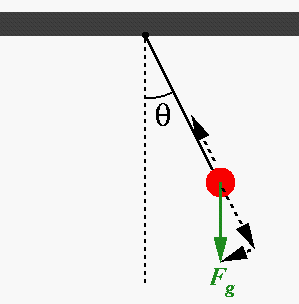
\includegraphics[width=0.5	\textwidth]{forcespend} \caption{Forças de gravidade $F_g$ no Pêndulo gravítico e a projecção na direção de movimento. \label{fig:3} } 
\end{figure}

Se o posição do pêndulo for descrita pela coordenada $s= l\; \theta$ ao longo da sua trajectória, 
então a força restauradora é 
\begin{equation}
	\label{eq:4} 
F_{tng} = - F_{g} \; sin(\theta) 
\end{equation}

E a equação diferencial de movimento 
\begin{align}
	\label{eq:5} 
	\frac{d^2 s}{dt^2} &=  l\;  \frac{d^2 \theta}{dt^2} \nonumber \\
	m \, l \, \frac{d^2 \theta}{dt^2} &= - m \,  g \, \sin(\theta)  \Rightarrow \frac{d^2 \theta}{dt^2} + \frac{g}{l} \sin(\theta) = 0
%l \,\frac{d^2 x}{dt^2} = \frac{k_{mola}}{m} x
\end{align}

Esta equação não tem uma resolução analítica simples, mas através do método  da \emph{linearização} (muito habitual na Física!), utiliza-se a aproximação $ \sin(\theta) \simeq \theta$ , para  $\theta_0 \ll 1$ (aqui  os angulos têm de ser medido em radianos!\footnote{ por exemplo: $\sin(5 ^{\circ}) = \sin(0.08726... \, \text{rad}) = 0.08715... $}).
Com esta aproximação ficamos com 

\begin{equation}
	\label{eq:6} 
	 \frac{d^2 \theta}{dt^2} + \frac{g}{l} \theta =0
\end{equation}

Cuja solução matemática é exacta e semelhante à expressão (\ref{eq:solu_mola})

\begin{equation}
	\label{eq:solu_pend}
\theta (t) = \theta_0 \sin(w_0 \, t + \phi_0) \text{, com } w_0 = \sqrt{\frac{g}{l}}
\end{equation}

O que é interessante neste modelo é que o efeito da \emph{massa gravítica } compensa o \emph{massa inercial } e portanto o período do pêndulo fica a  depender apenas do comprimento $l$  e do valor da aceleração da Gravidade $g$ no local 
\footnote{à superfície da Terra e à Latitude de Lisboa $g\approx 9.800\,m s^{-2}$.}
%à superfície da Terra $g\approx 9.81\,m s^{-2}$ e $g/\pi^2 \approx 0.994 \,m s^{-2}$}

\begin{equation}
	\label{eq:period_pend}
T_0 = \frac{2 \pi}{w_0} = 2\pi\; \sqrt{\frac{l}{g}} \text{, para }	\quad \theta_0 \ll 1
\end{equation}
%\simeq

Sabendo-se que já existiam pêndulos  desde a Antiguidade foi o génio  Galileo Galilei, que no início do séc. XVII os estudou detalhadamente, chegando relação (\ref{eq:period_pend}), sendo a partir daí 
estes dispositivos sistemáticamente utilizados para medir o tempo.

A resolução analítica da equação 	\ref{eq:5} (infelizmente bastante complexa) tem como solução para o período uma série  infinita de potências de $\theta_0$. 
Naturalmente, permite verificar que na aproximação $\theta_0 \ll 1$ a equação \ref{eq:period_pend} continua válida.
\begin{equation}
	\label{eq:period_pend_exa}
T_0 =  2\pi\, \sqrt{\frac{l}{g}} \left(1 + \frac{1}{16} \theta_0^{2} + \frac{11}{3072} \theta_0^{4} +
 \frac{737280}{3072} \theta_0^{6} + \frac{22931}{1321205760} \theta_0^{8} + \cdots \right)
\end{equation}

Até aqui desprezámos o atrito do ar no movimento do pêndulo. Ao introduzir esta contribuição, com a aproximação de atrito cinético 
proporcional à velocidade, a  equação	(\ref{eq:6}) muda para

\begin{equation}
%	\label{eq:6} 
	 \frac{d^2 \theta}{dt^2} + \lambda \, \frac{1}{m}  \frac{d \theta}{dt} + \frac{g}{l} \theta =0 \quad \lambda \text{ =Coeficiente de atrito viscoso}
\end{equation}

O primeiro efeito, que se pode verificar no laboratório é na amplitude do movimento $\theta_0$ que irá diminuir inexoravelmente com o tempo. 

O segundo efeito, muito mais difícil de observar, é que existe uma pequeníssima alteração no período $T$
\begin{equation}
T_1= T_0 / \sqrt{1 - \zeta^2} 
\end{equation}

Com $ \zeta = \frac{\lambda}{2\, m} \sqrt{\frac{l}{g}}  $

O factor  $ \zeta $ também pode relacionar com o factor de amortecimento $Q$ \footnote{Os Engenheiros chamam de factor de Qualidade} 
\begin{equation}
Q = 2 \pi \times \frac{\text{Energia do Pêndulo}}{\text{Energia perdida num ciclo}}
\end{equation}



%	 $\bullet$ Deflexão magnética em equilíbrio com deflexão eléctrica

%\textbf{Ver descrição no guia de laboratório pgs.77-81}

\end{document} 	

